\begin{enumerate}[label=\thechapter.\arabic*,ref=\thechapter.\theenumi]
\item A sinusoidal message signal having root mean square value of 4V and frequency of 1 kHz fed to a phase modulator with phase deviation constant 2 rad/volt. If the carrier signal is $c\brak{t} = 2\cos \brak{2\pi 10^6 t}$, the maximum instantaneous frequency of the phase modulated signal (rounded off to one decimal place) is \rule{1cm}{0.05mm} Hz. \hfill(GATE 2021 EC)\\
\solution\\
 \iffalse
\let\negmedspace\undefined
\let\negthickspace\undefined
\documentclass[journal,12pt,twocolumn]{IEEEtran}
\usepackage{amssymb}
\usepackage{cite}
\usepackage{amsmath,amssymb,amsfonts,amsthm}
\usepackage{algorithmic}
\usepackage{graphicx}
\usepackage{textcomp}
\usepackage{xcolor}
\usepackage{txfonts}
\usepackage{listings}
\usepackage{enumitem}
\usepackage{mathtools}
\usepackage{gensymb}
\usepackage{comment}
\usepackage[breaklinks=true]{hyperref}
\usepackage{tkz-euclide} 
\usepackage{listings}
\usepackage{gvv}                                        
\def\inputGnumericTable{}                                 
\usepackage[latin1]{inputenc}                                
\usepackage{color}                                            
\usepackage{array}                                            
\usepackage{longtable}                                       
\usepackage{calc}                                             
\usepackage{multirow}                                         
\usepackage{hhline}                                           
\usepackage{ifthen}                                           
\usepackage{lscape}
\usepackage{pgfplots}
\newtheorem{theorem}{Theorem}[section]
\newtheorem{problem}{Problem}
\newtheorem{proposition}{Proposition}[section]
\newtheorem{lemma}{Lemma}[section]
\newtheorem{corollary}[theorem]{Corollary}
\newtheorem{example}{Example}[section]
\newtheorem{definition}[problem]{Definition}
\newcommand{\BEQA}{\begin{eqnarray}}
\newcommand{\EEQA}{\end{eqnarray}}
\newcommand{\define}{\stackrel{\triangle}{=}}
\theoremstyle{remark}
\newtheorem{rem}{Remark}
\begin{document}

\bibliographystyle{IEEEtran}
\vspace{3cm}

\title{GATE.2021.EE.46}
\author{EE22BTECH11004 - Allu Lohith}

\maketitle
\newpage
\bigskip

\renewcommand{\thefigure}{\theenumi}
\renewcommand{\thetable}{\theenumi}

Consider a closed-loop system as shown, $$G_p\brak s= \frac{14.4}{s\brak{1+0.1s}}$$ is the plant transfer function and $G_c\brak s=1$ is the compensator. For a unit-step input, the output response has damped oscillations. The damped natural frequency is $\underline{\hspace{2cm}}$
$rad/s$. (Round off to 2 decimal places.)

\begin{figure}[h]
    \centering  
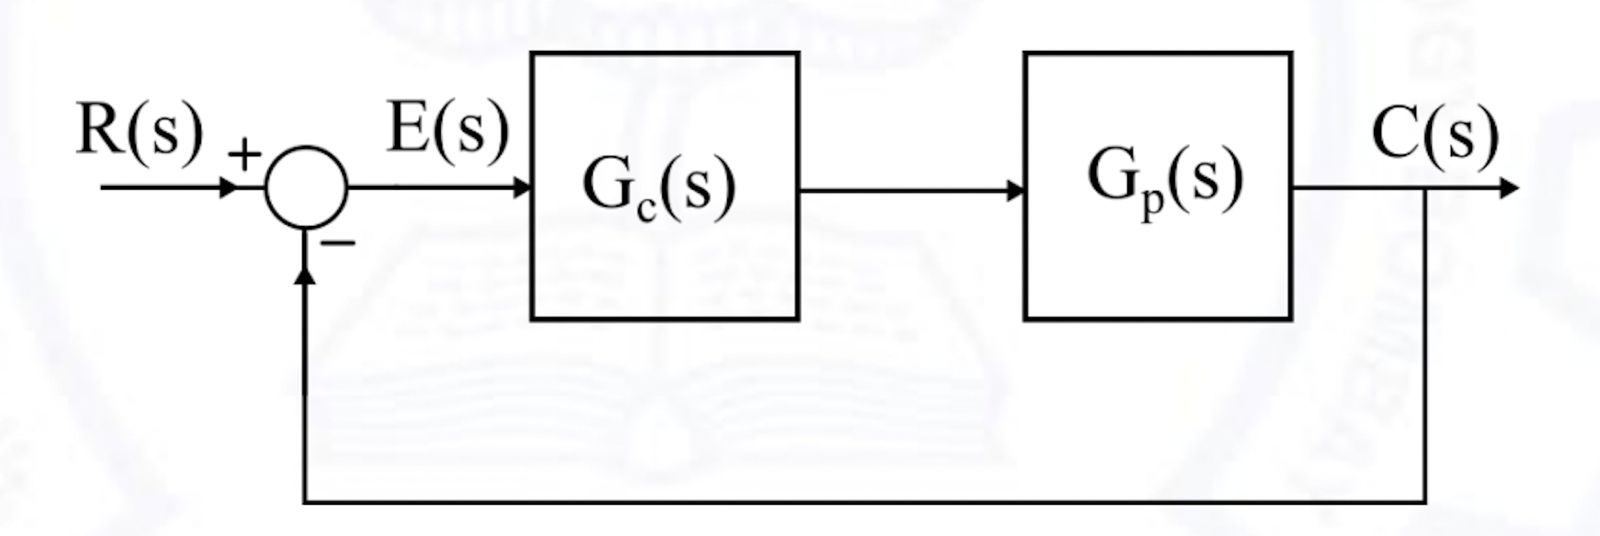
\includegraphics[width=\columnwidth]{2021/EE/46/figs/dia.png}
    \label{fig:ee.46.2021}
\end{figure}
\solution 
\fi
\begin{table}[h!]
\centering
\renewcommand{\arraystretch}{2}
\begin{tabular}{|p{2cm}|p{3cm}|p{2cm}|}
\hline 
\setlength{\tabcolsep}{1pt}
\textbf{Parameter}  &\textbf{Description} &\textbf{Value} \\
\hline
$G_n\brak s$ & Plant transfer function & $\dfrac{14.4}{s\brak{1+0.1s}}$ \\
\hline
$G_c\brak{s}$ &Transfer function of the compensator  & 1 \\
\hline
$\omega_n$ & Damped natural frequency& - \\
\hline
$T$& Overall tranfer function & $\dfrac{C}{R}$\\
\hline
\end{tabular}

\vspace{0.5cm}
\caption{\normalsize Parameters}
\end{table}
As we know that:
\begin{align}
E&=R_c-C_c\\
EG_cG_p&=C
\end{align}
So,
\begin{align}
E &= \frac{Cs\brak{1+0.1s}}{14.4}\\
\frac{Cs\brak{1+0.1s}}{14.4} &=R-C\\
R &=C\brak{\frac{s\brak{1+0.1s}}{14.4}+1}\\
\frac{C}{R} &= \frac{14.4}{0.1s^2+s+14.4}
\end{align}
The characteristic equation is $0.1s^2+s+14.4$ which is of the form $s^2 + 2\zeta\omega_n s + \omega_n^2$, So 
\begin{align}
    \omega_n^2&=144\\
    \omega_n&= 12rad/s
\end{align}

\begin{figure}[h]
    \centering  

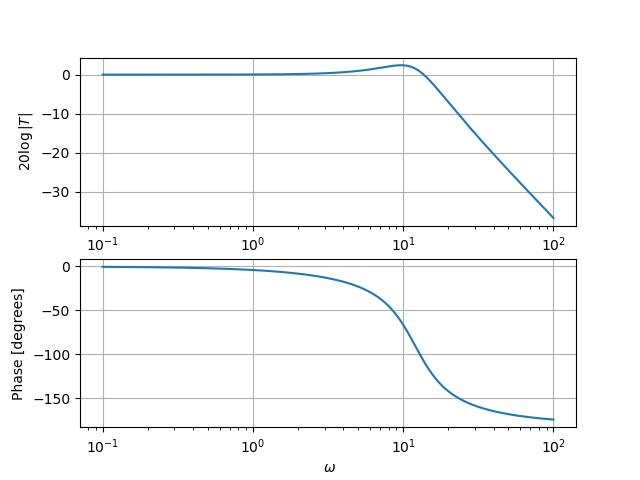
\includegraphics[width=\columnwidth]{2021/EE/46/figs/plot.png}

    \centering
    \caption{Bode Plot - Magnitude and Phase Response}

    \label{fig:ee2.46.2021}
\end{figure}



\pagebreak
\item Two discrete-time linear time-invarient systems with impulse responses $h_1[n]=\delta[n-1]+\delta[n+1]$ and $h_2[n]=\delta[n]+\delta[n-1]$ are connected in cascade, where $\delta[n]$ is the Kronecker delta. The impulse response of the cascaded system is   \\
\begin{enumerate}[label=(\alph*)]
    \item $\delta[n-2]+\delta[n+1]$
    \item $\delta[n-1]\delta[n]+\delta[n+1]\delta[n-1]$
    \item $\delta[n-2]+\delta[n-1]+\delta[n]+\delta[n+1]$
    \item $\delta[n]\delta[n-1]+\delta[n-2]\delta[n+1]$
\end{enumerate} \hfill(GATE 2021 EE)\\
\solution
\input{2021/EE/7/gate7.tex}
\pagebreak
\item Consider a superheterodyne receiver tuned to 600 kHz. If the local oscillator feeds a 1000 kHz signal to the mixer, the image frequency (in integer) is \underline{\hspace{1cm}} kHz.
\hfill(GATE EC 2021)\\
\solution
\input{2021/EC/50/50.tex}
\pagebreak
\item Consider a unity feedback system with closed loop transfer function
\begin{align*}
\frac{C\brak{s}}{R\brak{s}} &= \frac{s + 90}{s^2 + 10s + 90}
\end{align*}
The steady state error with respect to a unit ramp input is \rule{1cm}{0.15mm} .
\hfill(GATE 2021 BM) \\
\solution
 \iffalse
\let\negmedspace\undefined
\let\negthickspace\undefined
\documentclass[journal,12pt,twocolumn]{IEEEtran}
\usepackage{amssymb}
\usepackage{cite}
\usepackage{amsmath,amssymb,amsfonts,amsthm}
\usepackage{algorithmic}
\usepackage{graphicx}
\usepackage{textcomp}
\usepackage{xcolor}
\usepackage{txfonts}
\usepackage{listings}
\usepackage{enumitem}
\usepackage{mathtools}
\usepackage{gensymb}
\usepackage{comment}
\usepackage[breaklinks=true]{hyperref}
\usepackage{tkz-euclide} 
\usepackage{listings}
\usepackage{gvv}                                        
\def\inputGnumericTable{}                                 
\usepackage[latin1]{inputenc}                                
\usepackage{color}                                            
\usepackage{array}                                            
\usepackage{longtable}                                       
\usepackage{calc}                                             
\usepackage{multirow}                                         
\usepackage{hhline}                                           
\usepackage{ifthen}                                           
\usepackage{lscape}
\usepackage{pgfplots}
\newtheorem{theorem}{Theorem}[section]
\newtheorem{problem}{Problem}
\newtheorem{proposition}{Proposition}[section]
\newtheorem{lemma}{Lemma}[section]
\newtheorem{corollary}[theorem]{Corollary}
\newtheorem{example}{Example}[section]
\newtheorem{definition}[problem]{Definition}
\newcommand{\BEQA}{\begin{eqnarray}}
\newcommand{\EEQA}{\end{eqnarray}}
\newcommand{\define}{\stackrel{\triangle}{=}}
\theoremstyle{remark}
\newtheorem{rem}{Remark}
\begin{document}

\bibliographystyle{IEEEtran}
\vspace{3cm}

\title{GATE.2021.EE.46}
\author{EE22BTECH11004 - Allu Lohith}

\maketitle
\newpage
\bigskip

\renewcommand{\thefigure}{\theenumi}
\renewcommand{\thetable}{\theenumi}

Consider a closed-loop system as shown, $$G_p\brak s= \frac{14.4}{s\brak{1+0.1s}}$$ is the plant transfer function and $G_c\brak s=1$ is the compensator. For a unit-step input, the output response has damped oscillations. The damped natural frequency is $\underline{\hspace{2cm}}$
$rad/s$. (Round off to 2 decimal places.)

\begin{figure}[h]
    \centering  
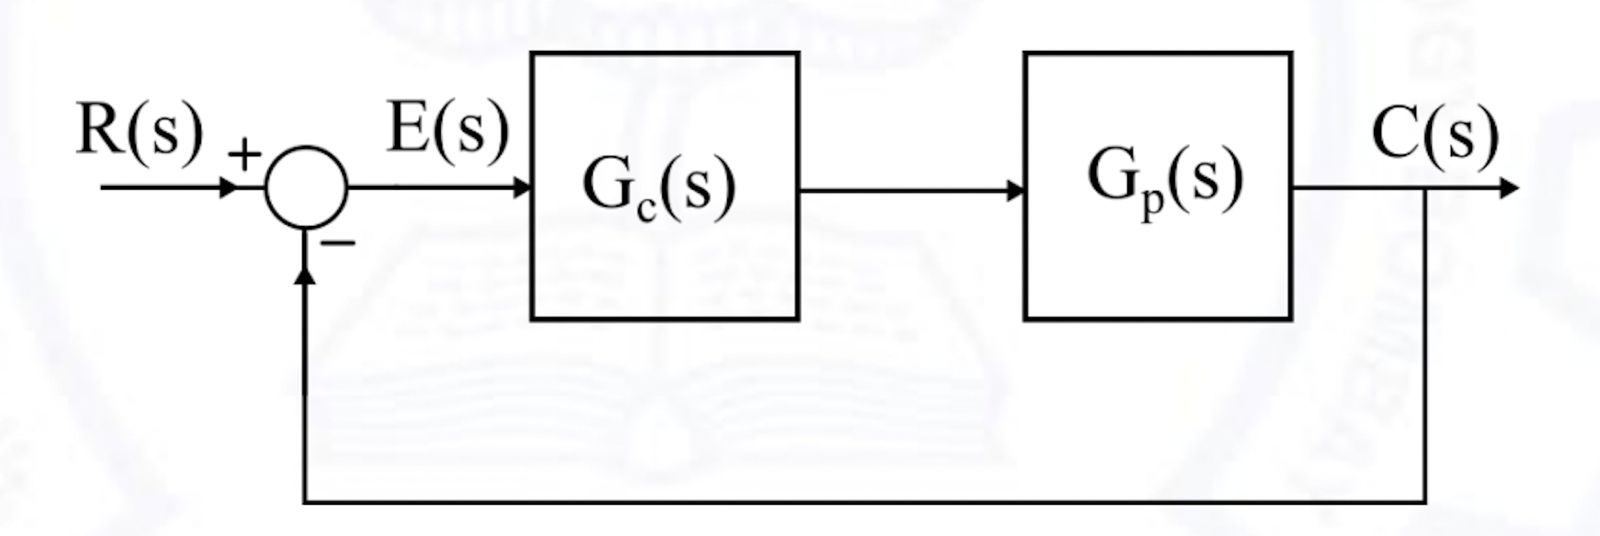
\includegraphics[width=\columnwidth]{2021/EE/46/figs/dia.png}
    \label{fig:ee.46.2021}
\end{figure}
\solution 
\fi
\begin{table}[h!]
\centering
\renewcommand{\arraystretch}{2}
\begin{tabular}{|p{2cm}|p{3cm}|p{2cm}|}
\hline 
\setlength{\tabcolsep}{1pt}
\textbf{Parameter}  &\textbf{Description} &\textbf{Value} \\
\hline
$G_n\brak s$ & Plant transfer function & $\dfrac{14.4}{s\brak{1+0.1s}}$ \\
\hline
$G_c\brak{s}$ &Transfer function of the compensator  & 1 \\
\hline
$\omega_n$ & Damped natural frequency& - \\
\hline
$T$& Overall tranfer function & $\dfrac{C}{R}$\\
\hline
\end{tabular}

\vspace{0.5cm}
\caption{\normalsize Parameters}
\end{table}
As we know that:
\begin{align}
E&=R_c-C_c\\
EG_cG_p&=C
\end{align}
So,
\begin{align}
E &= \frac{Cs\brak{1+0.1s}}{14.4}\\
\frac{Cs\brak{1+0.1s}}{14.4} &=R-C\\
R &=C\brak{\frac{s\brak{1+0.1s}}{14.4}+1}\\
\frac{C}{R} &= \frac{14.4}{0.1s^2+s+14.4}
\end{align}
The characteristic equation is $0.1s^2+s+14.4$ which is of the form $s^2 + 2\zeta\omega_n s + \omega_n^2$, So 
\begin{align}
    \omega_n^2&=144\\
    \omega_n&= 12rad/s
\end{align}

\begin{figure}[h]
    \centering  

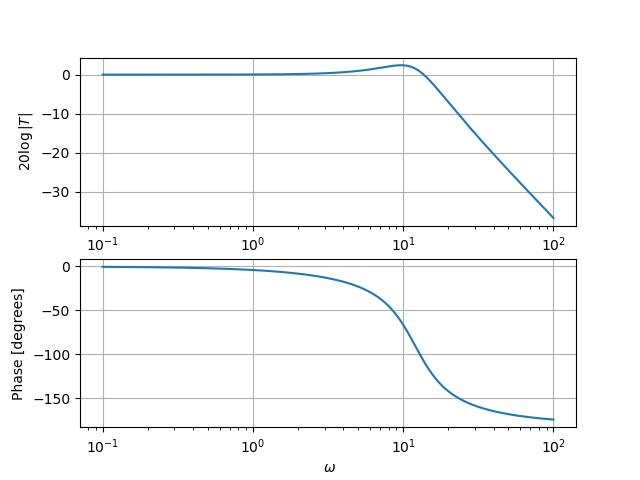
\includegraphics[width=\columnwidth]{2021/EE/46/figs/plot.png}

    \centering
    \caption{Bode Plot - Magnitude and Phase Response}

    \label{fig:ee2.46.2021}
\end{figure}



\item A unit step input is applied to a system with impulse response H\brak{s} = $\frac{1- \frac{s}{\omega{_z}}}{1+\frac{s}{\omega{_p}}}$ at t=0. The output of the system $y\brak{t}$ at t=$0^+$ is:
\begin{enumerate}[label=\alph*)]
 \item 1
 \item $-\frac{\omega{_z}}{\omega{_p}}$
 \item $-\frac{\omega{_p}}{\omega{_z}}$
 \item 0
\end{enumerate} \hfill(GATE 2021 BM)\\
\solution
\input{2021/BM/27/27.tex}

\item In the block diagram shown below, an infinite tap FIR filter with transfer function $H\brak{z}=\frac{Y\brak{z}}{X\brak{z}}$ is realized. If $H\brak{z}=\frac{1}{1-0.5z^{-1}}$.\\the value of $\alpha$ is
\begin{figure}[h]
    \includegraphics[width=1\columnwidth]{2021/BM/31/figs/questionfig.png}
    \label{fig:question31bm}
\end{figure} \hfill(GATE 2021 BM)\\
\solution
\input{2021/BM/31/Assignmentbm31.tex}
\pagebreak
\item A unity feedback system that uses proportional-integral (PI) control is shown in the figure.
 \begin{figure}[!ht]    
    \centering
\graphicspath{ {2021/EC/48/figs} }
\includegraphics[width=\columnwidth]{figure_1}
\label{figure:ee25-gate4-graph}
\end{figure}
The stability of the overall system is controlled by tuning the PI control parameters $K_p$ and $K_i$. The maximum value of $K_i$ that can be chosen so as to keep the overall system stable or, in the worst case, marginally stable (\textit{rounded off to three decimal places}) is?
\hfill{(GATE EC 2021)}\\
\solution
\input{2021/EC/48/ec-48.tex}
\pagebreak
\item In the given figure, plant $G_p(s)=\frac{2.2}{(1+0.1s)(1+0.4s)(1+1.2s)}$ and compensator $G_c(s)=K\brak{\frac{1+T_1s}{1+T_2s}}$ . The external disturbance input is D(s). It is desired that when the disturbance is a unit step, the steady-state error should not exceed 0.1 unit. The minimum value of K is 
\hfill{(GATE EE 2021)}\\
\begin{figure}[h!]
    \centering
    \includegraphics[width=\columnwidth]{2021/EE/47/figs/fig.png}
    \caption{}
    \label{fig:sr40}
\end{figure}
\\
\solution
\input{2021/EE/47/gate.tex}
\pagebreak
\item For the closed loop system shown , the transfer function $\frac{E(s)}{R(s)}$ is \\
\begin{figure}[ht]
	\centering
	\includegraphics[width=1\linewidth]{2021/EE/11/figs/questiondia.png}
\end{figure}
\begin{enumerate}[label = (\alph*)]
	\item $\frac{G}{1+GH}$
	\item $\frac{GH}{1+GH}$
	\item $\frac{1}{1+GH}$
	\item $\frac{1}{1+G}$
\end{enumerate} \hfill{(GATE EE 2021)}\\
 \iffalse
\let\negmedspace\undefined
\let\negthickspace\undefined
\documentclass[journal,12pt,twocolumn]{IEEEtran}
\usepackage{amssymb}
\usepackage{cite}
\usepackage{amsmath,amssymb,amsfonts,amsthm}
\usepackage{algorithmic}
\usepackage{graphicx}
\usepackage{textcomp}
\usepackage{xcolor}
\usepackage{txfonts}
\usepackage{listings}
\usepackage{enumitem}
\usepackage{mathtools}
\usepackage{gensymb}
\usepackage{comment}
\usepackage[breaklinks=true]{hyperref}
\usepackage{tkz-euclide} 
\usepackage{listings}
\usepackage{gvv}                                        
\def\inputGnumericTable{}                                 
\usepackage[latin1]{inputenc}                                
\usepackage{color}                                            
\usepackage{array}                                            
\usepackage{longtable}                                       
\usepackage{calc}                                             
\usepackage{multirow}                                         
\usepackage{hhline}                                           
\usepackage{ifthen}                                           
\usepackage{lscape}
\usepackage{pgfplots}
\newtheorem{theorem}{Theorem}[section]
\newtheorem{problem}{Problem}
\newtheorem{proposition}{Proposition}[section]
\newtheorem{lemma}{Lemma}[section]
\newtheorem{corollary}[theorem]{Corollary}
\newtheorem{example}{Example}[section]
\newtheorem{definition}[problem]{Definition}
\newcommand{\BEQA}{\begin{eqnarray}}
\newcommand{\EEQA}{\end{eqnarray}}
\newcommand{\define}{\stackrel{\triangle}{=}}
\theoremstyle{remark}
\newtheorem{rem}{Remark}
\begin{document}

\bibliographystyle{IEEEtran}
\vspace{3cm}

\title{GATE.2021.EE.46}
\author{EE22BTECH11004 - Allu Lohith}

\maketitle
\newpage
\bigskip

\renewcommand{\thefigure}{\theenumi}
\renewcommand{\thetable}{\theenumi}

Consider a closed-loop system as shown, $$G_p\brak s= \frac{14.4}{s\brak{1+0.1s}}$$ is the plant transfer function and $G_c\brak s=1$ is the compensator. For a unit-step input, the output response has damped oscillations. The damped natural frequency is $\underline{\hspace{2cm}}$
$rad/s$. (Round off to 2 decimal places.)

\begin{figure}[h]
    \centering  
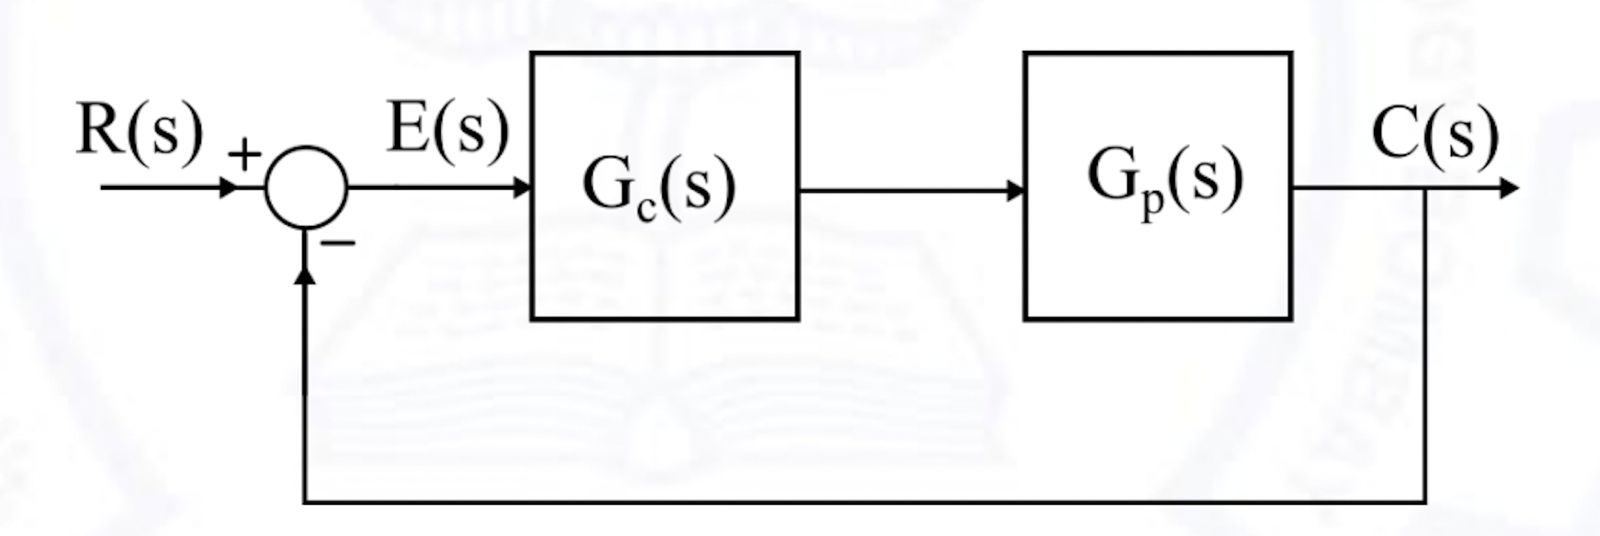
\includegraphics[width=\columnwidth]{2021/EE/46/figs/dia.png}
    \label{fig:ee.46.2021}
\end{figure}
\solution 
\fi
\begin{table}[h!]
\centering
\renewcommand{\arraystretch}{2}
\begin{tabular}{|p{2cm}|p{3cm}|p{2cm}|}
\hline 
\setlength{\tabcolsep}{1pt}
\textbf{Parameter}  &\textbf{Description} &\textbf{Value} \\
\hline
$G_n\brak s$ & Plant transfer function & $\dfrac{14.4}{s\brak{1+0.1s}}$ \\
\hline
$G_c\brak{s}$ &Transfer function of the compensator  & 1 \\
\hline
$\omega_n$ & Damped natural frequency& - \\
\hline
$T$& Overall tranfer function & $\dfrac{C}{R}$\\
\hline
\end{tabular}

\vspace{0.5cm}
\caption{\normalsize Parameters}
\end{table}
As we know that:
\begin{align}
E&=R_c-C_c\\
EG_cG_p&=C
\end{align}
So,
\begin{align}
E &= \frac{Cs\brak{1+0.1s}}{14.4}\\
\frac{Cs\brak{1+0.1s}}{14.4} &=R-C\\
R &=C\brak{\frac{s\brak{1+0.1s}}{14.4}+1}\\
\frac{C}{R} &= \frac{14.4}{0.1s^2+s+14.4}
\end{align}
The characteristic equation is $0.1s^2+s+14.4$ which is of the form $s^2 + 2\zeta\omega_n s + \omega_n^2$, So 
\begin{align}
    \omega_n^2&=144\\
    \omega_n&= 12rad/s
\end{align}

\begin{figure}[h]
    \centering  

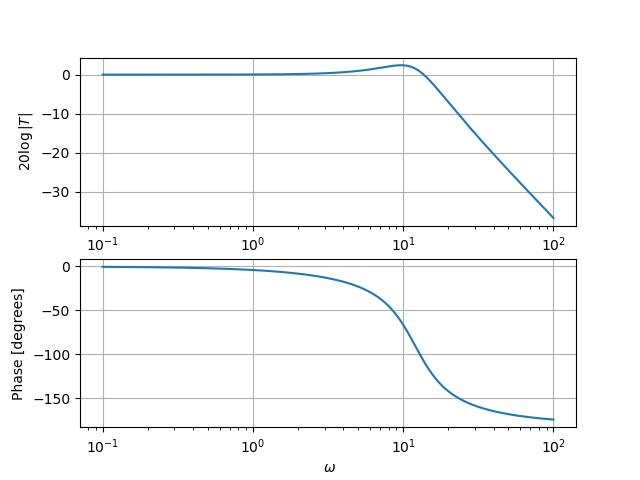
\includegraphics[width=\columnwidth]{2021/EE/46/figs/plot.png}

    \centering
    \caption{Bode Plot - Magnitude and Phase Response}

    \label{fig:ee2.46.2021}
\end{figure}



\pagebreak

Consider two 16-point sequences x\sbrak{n} and h\sbrak{n}. Let the linear convolution of x\sbrak{n} and h\sbrak{n} be denoted by y\sbrak{n}, while z\sbrak{n} denotes the 16-point inverse discrete Fourier transform \brak{IDFT} of the product of the 16-point DFTs of x\brak{n} and h\sbrak{n}. The values of k for which z\sbrak{k} = y\sbrak{k} are 
\begin{enumerate}
    \item $k = 0, 1, 2, 3, ... , 15$
    \item $k = 0$
    \item $k = 15$
    \item $k = 0$ and $k = 15$
\end{enumerate}
\hfill(GATE EC 2021)\\
\solution
\input{2021/EC/5/ec5.tex}
\pagebreak
\item The input signal shown below \\
\input{2021/IN/44/figs/xn}\\
is passed through the filter with following taps\\
\input{2021/IN/44/figs/n}\\
The number of non-zero output samples is \underline{\hspace{1cm}}.\\
\hfill(GATE IN 2021)
\solution
 \iffalse
\let\negmedspace\undefined
\let\negthickspace\undefined
\documentclass[journal,12pt,twocolumn]{IEEEtran}
\usepackage{amssymb}
\usepackage{cite}
\usepackage{amsmath,amssymb,amsfonts,amsthm}
\usepackage{algorithmic}
\usepackage{graphicx}
\usepackage{textcomp}
\usepackage{xcolor}
\usepackage{txfonts}
\usepackage{listings}
\usepackage{enumitem}
\usepackage{mathtools}
\usepackage{gensymb}
\usepackage{comment}
\usepackage[breaklinks=true]{hyperref}
\usepackage{tkz-euclide} 
\usepackage{listings}
\usepackage{gvv}                                        
\def\inputGnumericTable{}                                 
\usepackage[latin1]{inputenc}                                
\usepackage{color}                                            
\usepackage{array}                                            
\usepackage{longtable}                                       
\usepackage{calc}                                             
\usepackage{multirow}                                         
\usepackage{hhline}                                           
\usepackage{ifthen}                                           
\usepackage{lscape}
\usepackage{pgfplots}
\newtheorem{theorem}{Theorem}[section]
\newtheorem{problem}{Problem}
\newtheorem{proposition}{Proposition}[section]
\newtheorem{lemma}{Lemma}[section]
\newtheorem{corollary}[theorem]{Corollary}
\newtheorem{example}{Example}[section]
\newtheorem{definition}[problem]{Definition}
\newcommand{\BEQA}{\begin{eqnarray}}
\newcommand{\EEQA}{\end{eqnarray}}
\newcommand{\define}{\stackrel{\triangle}{=}}
\theoremstyle{remark}
\newtheorem{rem}{Remark}
\begin{document}

\bibliographystyle{IEEEtran}
\vspace{3cm}

\title{GATE.2021.EE.46}
\author{EE22BTECH11004 - Allu Lohith}

\maketitle
\newpage
\bigskip

\renewcommand{\thefigure}{\theenumi}
\renewcommand{\thetable}{\theenumi}

Consider a closed-loop system as shown, $$G_p\brak s= \frac{14.4}{s\brak{1+0.1s}}$$ is the plant transfer function and $G_c\brak s=1$ is the compensator. For a unit-step input, the output response has damped oscillations. The damped natural frequency is $\underline{\hspace{2cm}}$
$rad/s$. (Round off to 2 decimal places.)

\begin{figure}[h]
    \centering  
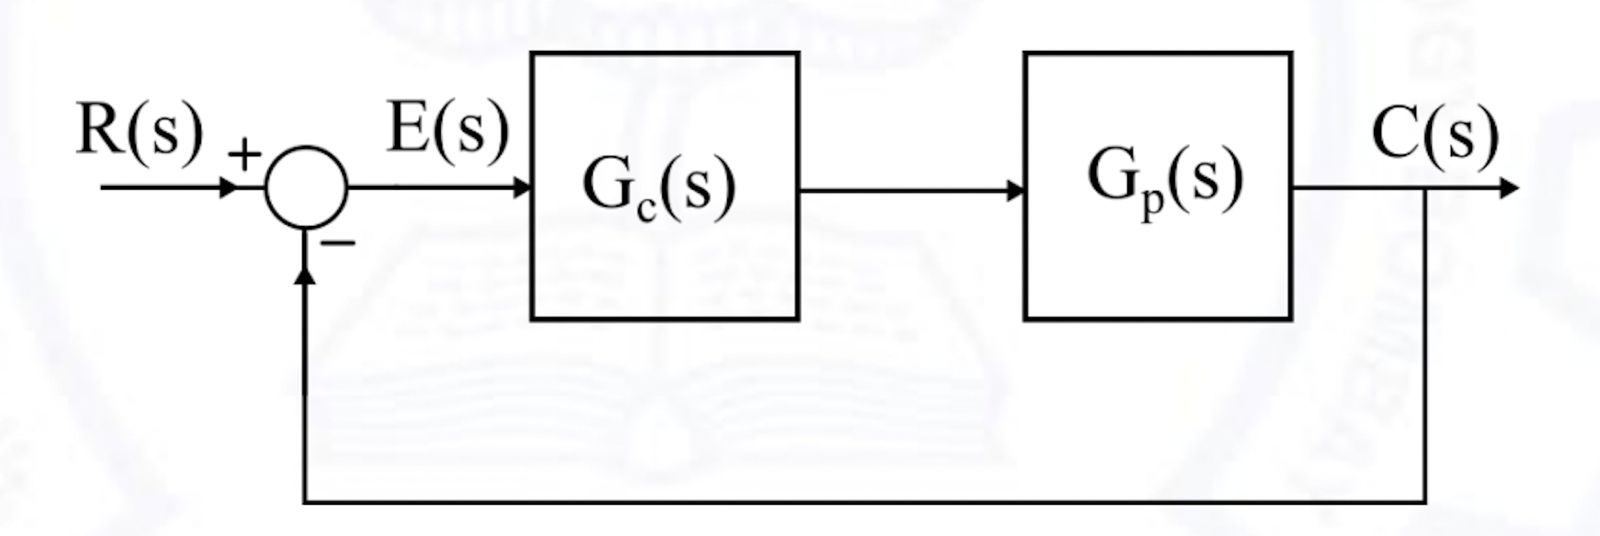
\includegraphics[width=\columnwidth]{2021/EE/46/figs/dia.png}
    \label{fig:ee.46.2021}
\end{figure}
\solution 
\fi
\begin{table}[h!]
\centering
\renewcommand{\arraystretch}{2}
\begin{tabular}{|p{2cm}|p{3cm}|p{2cm}|}
\hline 
\setlength{\tabcolsep}{1pt}
\textbf{Parameter}  &\textbf{Description} &\textbf{Value} \\
\hline
$G_n\brak s$ & Plant transfer function & $\dfrac{14.4}{s\brak{1+0.1s}}$ \\
\hline
$G_c\brak{s}$ &Transfer function of the compensator  & 1 \\
\hline
$\omega_n$ & Damped natural frequency& - \\
\hline
$T$& Overall tranfer function & $\dfrac{C}{R}$\\
\hline
\end{tabular}

\vspace{0.5cm}
\caption{\normalsize Parameters}
\end{table}
As we know that:
\begin{align}
E&=R_c-C_c\\
EG_cG_p&=C
\end{align}
So,
\begin{align}
E &= \frac{Cs\brak{1+0.1s}}{14.4}\\
\frac{Cs\brak{1+0.1s}}{14.4} &=R-C\\
R &=C\brak{\frac{s\brak{1+0.1s}}{14.4}+1}\\
\frac{C}{R} &= \frac{14.4}{0.1s^2+s+14.4}
\end{align}
The characteristic equation is $0.1s^2+s+14.4$ which is of the form $s^2 + 2\zeta\omega_n s + \omega_n^2$, So 
\begin{align}
    \omega_n^2&=144\\
    \omega_n&= 12rad/s
\end{align}

\begin{figure}[h]
    \centering  

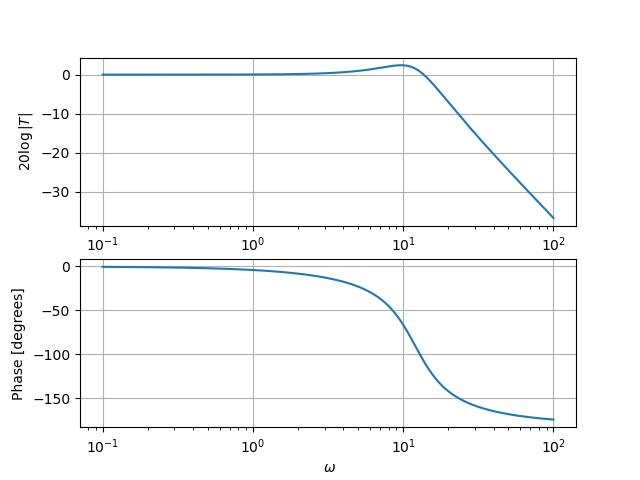
\includegraphics[width=\columnwidth]{2021/EE/46/figs/plot.png}

    \centering
    \caption{Bode Plot - Magnitude and Phase Response}

    \label{fig:ee2.46.2021}
\end{figure}



\pagebreak
\item A sinusoid $(\sqrt{2}sin(t))\mu(t)$,where $\mu(t)$ is the step input,is applied to a system with transfer function G(s)=$\frac{1}{1+s}$.The amplitude of the steady state output is\hfill{(GATE IN 2021)}\\
\solution
\input{2021/IN/45/gate21.in.45.tex}
\pagebreak
\item The block diagram of a feedback control system is shown in the figure .
\begin{center}
\includegraphics[width=0.5\textwidth]{2021/EC/13/figs/figure1.png}
\end{center}
The transfer function $\frac{Y(s)}{X(s)}$ of the system is :
\hfill(GATE 2021 EC)\\
\solution
\input{2021/EC/13/ec13.tex}
\pagebreak
\item Consider a unity feedback configuration with a plant and a PID controller as shown in the figure. $G(s) = \frac{1}{(s+1)(s+3)} $ and $ C(s) = \frac{K(s+3+j)(s+3-j)}{s}$ with K being scalar . The closed loop is :
\begin{center}
\includegraphics[width=0.5\textwidth]{2021/IN/29/figs/figure1.jpg}
\end{center}
\begin{enumerate}
\item[A]only stable for $K < 0$
\item[B]stable for all value of K
\item[C]only stable for $K > 0$
\item[D]only stable for K between –1 and +1
\end{enumerate}
\hfill(GATE 2021 IN)\\
\solution
\input{2021/IN/29/in29.tex}
\pagebreak
\item Consider a closed-loop system as shown, $$G_p\brak s= \frac{14.4}{s\brak{1+0.1s}}$$ is the plant transfer function and $G_c\brak s=1$ is the compensator. For a unit-step input, the output response has damped oscillations. The damped natural frequency is $\underline{\hspace{2cm}}$
$rad/s$. (Round off to 2 decimal places.) 
\hfill(GATE EE 46 2021)

\begin{figure}[h]
    \centering  
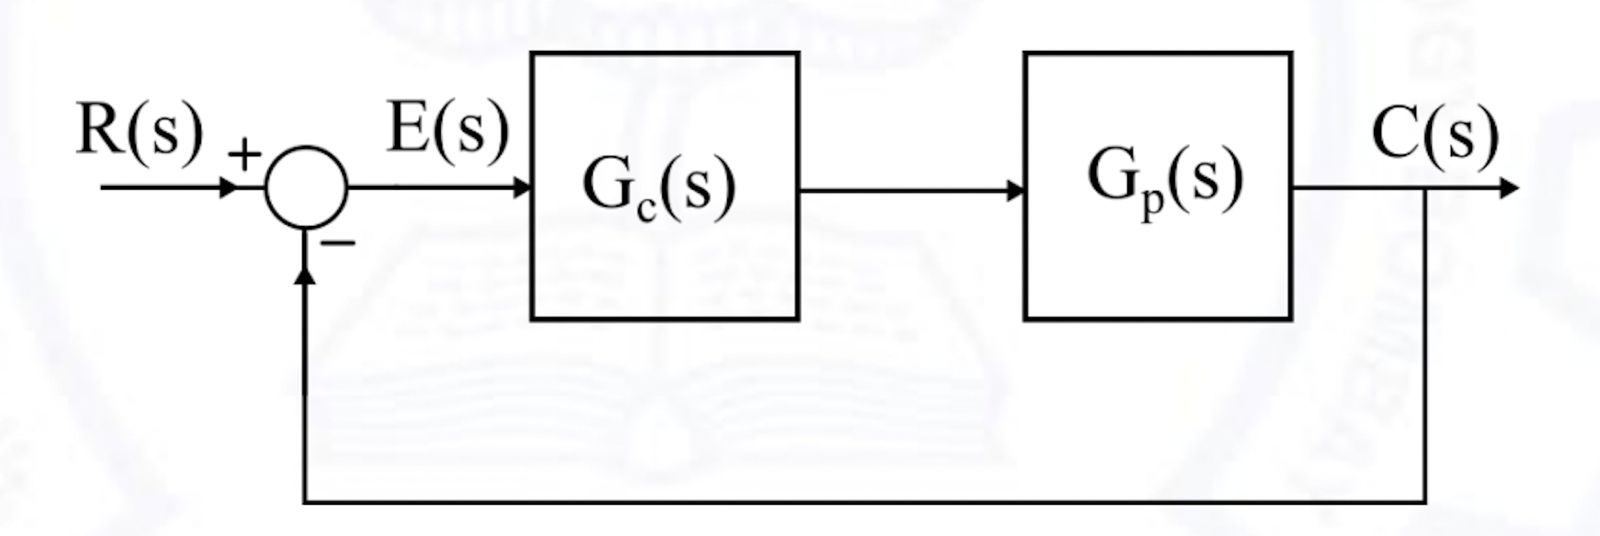
\includegraphics[width=\columnwidth]{2021/EE/46/figs/dia.png}
    \label{fig:ee.46.2021}
\end{figure}
\solution 
 \iffalse
\let\negmedspace\undefined
\let\negthickspace\undefined
\documentclass[journal,12pt,twocolumn]{IEEEtran}
\usepackage{amssymb}
\usepackage{cite}
\usepackage{amsmath,amssymb,amsfonts,amsthm}
\usepackage{algorithmic}
\usepackage{graphicx}
\usepackage{textcomp}
\usepackage{xcolor}
\usepackage{txfonts}
\usepackage{listings}
\usepackage{enumitem}
\usepackage{mathtools}
\usepackage{gensymb}
\usepackage{comment}
\usepackage[breaklinks=true]{hyperref}
\usepackage{tkz-euclide} 
\usepackage{listings}
\usepackage{gvv}                                        
\def\inputGnumericTable{}                                 
\usepackage[latin1]{inputenc}                                
\usepackage{color}                                            
\usepackage{array}                                            
\usepackage{longtable}                                       
\usepackage{calc}                                             
\usepackage{multirow}                                         
\usepackage{hhline}                                           
\usepackage{ifthen}                                           
\usepackage{lscape}
\usepackage{pgfplots}
\newtheorem{theorem}{Theorem}[section]
\newtheorem{problem}{Problem}
\newtheorem{proposition}{Proposition}[section]
\newtheorem{lemma}{Lemma}[section]
\newtheorem{corollary}[theorem]{Corollary}
\newtheorem{example}{Example}[section]
\newtheorem{definition}[problem]{Definition}
\newcommand{\BEQA}{\begin{eqnarray}}
\newcommand{\EEQA}{\end{eqnarray}}
\newcommand{\define}{\stackrel{\triangle}{=}}
\theoremstyle{remark}
\newtheorem{rem}{Remark}
\begin{document}

\bibliographystyle{IEEEtran}
\vspace{3cm}

\title{GATE.2021.EE.46}
\author{EE22BTECH11004 - Allu Lohith}

\maketitle
\newpage
\bigskip

\renewcommand{\thefigure}{\theenumi}
\renewcommand{\thetable}{\theenumi}

Consider a closed-loop system as shown, $$G_p\brak s= \frac{14.4}{s\brak{1+0.1s}}$$ is the plant transfer function and $G_c\brak s=1$ is the compensator. For a unit-step input, the output response has damped oscillations. The damped natural frequency is $\underline{\hspace{2cm}}$
$rad/s$. (Round off to 2 decimal places.)

\begin{figure}[h]
    \centering  
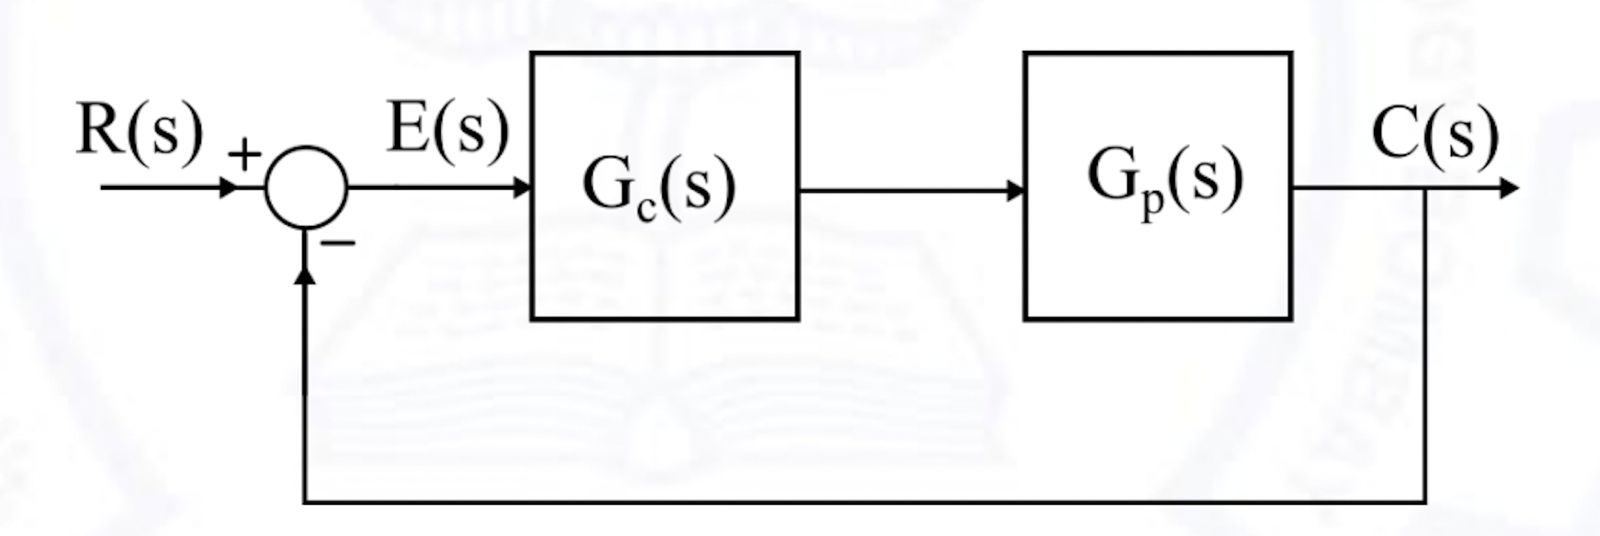
\includegraphics[width=\columnwidth]{2021/EE/46/figs/dia.png}
    \label{fig:ee.46.2021}
\end{figure}
\solution 
\fi
\begin{table}[h!]
\centering
\renewcommand{\arraystretch}{2}
\begin{tabular}{|p{2cm}|p{3cm}|p{2cm}|}
\hline 
\setlength{\tabcolsep}{1pt}
\textbf{Parameter}  &\textbf{Description} &\textbf{Value} \\
\hline
$G_n\brak s$ & Plant transfer function & $\dfrac{14.4}{s\brak{1+0.1s}}$ \\
\hline
$G_c\brak{s}$ &Transfer function of the compensator  & 1 \\
\hline
$\omega_n$ & Damped natural frequency& - \\
\hline
$T$& Overall tranfer function & $\dfrac{C}{R}$\\
\hline
\end{tabular}

\vspace{0.5cm}
\caption{\normalsize Parameters}
\end{table}
As we know that:
\begin{align}
E&=R_c-C_c\\
EG_cG_p&=C
\end{align}
So,
\begin{align}
E &= \frac{Cs\brak{1+0.1s}}{14.4}\\
\frac{Cs\brak{1+0.1s}}{14.4} &=R-C\\
R &=C\brak{\frac{s\brak{1+0.1s}}{14.4}+1}\\
\frac{C}{R} &= \frac{14.4}{0.1s^2+s+14.4}
\end{align}
The characteristic equation is $0.1s^2+s+14.4$ which is of the form $s^2 + 2\zeta\omega_n s + \omega_n^2$, So 
\begin{align}
    \omega_n^2&=144\\
    \omega_n&= 12rad/s
\end{align}

\begin{figure}[h]
    \centering  

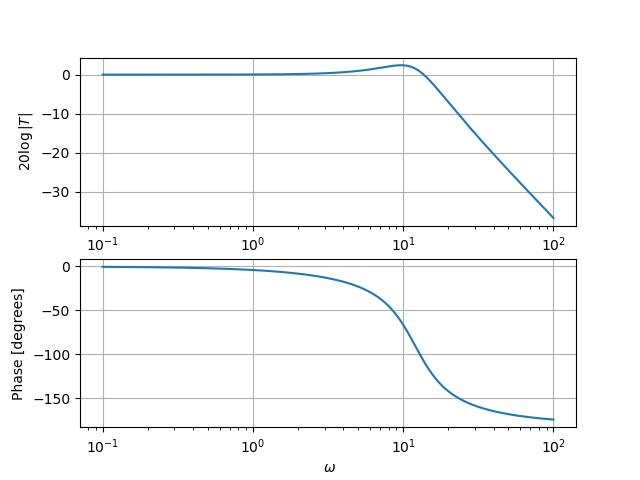
\includegraphics[width=\columnwidth]{2021/EE/46/figs/plot.png}

    \centering
    \caption{Bode Plot - Magnitude and Phase Response}

    \label{fig:ee2.46.2021}
\end{figure}



\pagebreak

\item  For a linear stable second order system, if the unit step response is such that peak time is twice the rise time, then the system is . 
    \begin{enumerate}
    \item underdamped\\
    \item undamped\\
    \item overdamped\\
    \item critically damped\\
    \end{enumerate} \hfill(GATE BM 8 2021)\\
    \solution
    
\documentclass[journal,12pt,onecolumn]{IEEEtran}
\usepackage{cite}
\usepackage{amsmath,amssymb,amsfonts,amsthm}
\usepackage{algorithmic}
\usepackage{graphicx}
\usepackage{textcomp}
\usepackage{xcolor}
\usepackage{txfonts}
\usepackage{listings}
\usepackage{enumitem}
\usepackage{mathtools}
\usepackage{gensymb}
\usepackage{comment}
\usepackage[breaklinks=true]{hyperref}
\usepackage{tkz-euclide}
\usepackage{listings}
\usepackage{gvv}
\def\inputGnumericTable{}
\usepackage[latin1]{inputenc}
\usepackage{color}
\usepackage{array}
\usepackage{longtable}
\usepackage{calc}
\usepackage{multirow}
\usepackage{hhline}
\usepackage{ifthen}
\usepackage{lscape}

\newtheorem{theorem}{Theorem}[section]
\newtheorem{problem}{Problem}
\newtheorem{proposition}{Proposition}[section]
\newtheorem{lemma}{Lemma}[section]
\newtheorem{corollary}[theorem]{Corollary}
\newtheorem{example}{Example}[section]
\newtheorem{definition}[problem]{Definition}
\newcommand{\BEQA}{\begin{eqnarray}}
    \newcommand{\EEQA}{\end{eqnarray}}
\newcommand{\define}{\stackrel{\triangle}{=}}
\theoremstyle{remark}
\newtheorem{rem}{Remark}

\begin{document}
    
    \bibliographystyle{IEEEtran}
    \vspace{3cm}
    
    \title{Gate 2021 BM Q8}
    \author{EE23BTECH11212 - Manugunta Meghana Sai$^{*}$% <-this % stops a space
    }
    \maketitle
    \bigskip
    
    \renewcommand{\thefigure}{\theenumi}
    \renewcommand{\thetable}{\theenumi}
    
    \vspace{3cm}
    
    For a linear stable second order system, if the unit step response is such that peak time is twice the rise time, then the system is . 
    \begin{enumerate}
    \item underdamped\\
    \item undamped\\
    \item overdamped\\
    \item critically damped\\
    \end{enumerate}
    \solution
    \begin{table}[h!]
 	\centering
 	\resizebox{6 cm}{!}{
 		\renewcommand{\arraystretch}{2}
\begin{tabular}{|p{2cm}|p{3cm}|p{2cm}|}
\hline 
\setlength{\tabcolsep}{1pt}
\textbf{Parameter}  &\textbf{Description} &\textbf{Value} \\
\hline
$G_n\brak s$ & Plant transfer function & $\dfrac{14.4}{s\brak{1+0.1s}}$ \\
\hline
$G_c\brak{s}$ &Transfer function of the compensator  & 1 \\
\hline
$\omega_n$ & Damped natural frequency& - \\
\hline
$T$& Overall tranfer function & $\dfrac{C}{R}$\\
\hline
\end{tabular}

 	}
 	\caption{Given Parameters}
 	\label{tab:msmBMgate8tab1}
     \end{table} 
    \\The rise time is given by:
    \begin{align}
    t_{r} = \frac{\pi-\theta}{\omega_{n} \sqrt{1-\zeta^{2}}}
    \end{align}
    The peak time is given by:
    \begin{align}
    t_{p} = \frac{\pi}{\omega_{n} \sqrt{1-\zeta^{2}}}
    \end{align}
    as, peak time is twice the rise time:
    \begin{align}
    t_{p} &= 2t_{r}\\
    \frac{\pi}{\omega_{n} \sqrt{1-\zeta^{2}}} &= 2\frac{\pi-\theta}{\omega_{n} \sqrt{1-\zeta^{2}}}\\
    \theta &= \frac{\pi}{2}
    \end{align}
    as, $\theta = \frac{\pi}{2}$, both roots of the system are imaginary, so 
    \begin{align}
    G\brak{s} = \frac{\omega_n^2}{s^2 + 2\zeta\omega_n s + \omega_n^2}
    \end{align}
    So, for the denominator to have two imaginary roots
    \begin{align}
      s = +\j\omega_{n}\\
      s = -\j\omega_{n}
    \end{align}
     $2\zeta\omega_n$ should be zero.
   
    \begin{align}
    \zeta = 0
    \end{align}
    The Routh-Hurwitz criterion is a method used to determine the stability of a system based on the locations of the roots of the characteristic equation in the complex plane.\\
    
     The coefficients of $s$, $s^{2}$ and 1, which are $2\zeta \omega_{n}$, $1$ and $\omega_{n}^{2}$ are non negative, hence the system is stable.So,the syatem is either undamped or overdamped.As, 
    $\zeta$ is zero, system is undamped. 
\end{document}

\end{enumerate}
